\section{Scenarios} \label{sec:scenarios}

In this section, we will explain different scenarios happening during the image capture, that affect how the object appears in the image. Scenarios depend on the mode of tracking (sidereal, object) and the relative velocity between the moving object of interest and the telescope. 

\subsection{Point-like stars, point-like objects}
This is a typical scenario occurring in astronomical images and is shown in the Figure \ref{fig:pointpoint1}. The angular velocity of the moving object of interest is so small that during the exposure time their position on the image doesn't seem to move. The speed is so slow that they don't cross more than one pixel, which leads to the appearance of the object as a point. This applies to both, objects of interest as well as stars. 

This scenario commonly happens in an asteroid field, small solar body system field, and can also appear in space-debris observations when high cadence and low exposure time is used. 

\begin{figure}[!h]
    \centering
    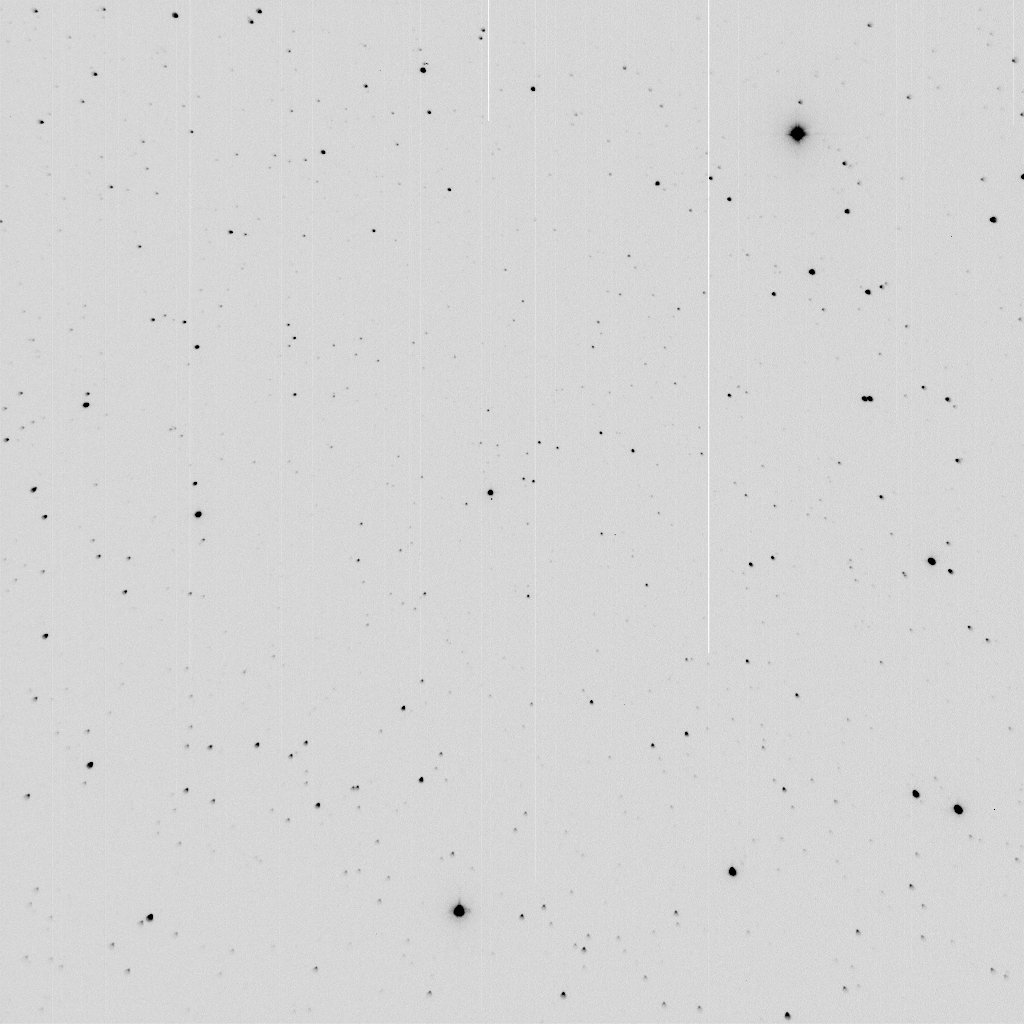
\includegraphics[width=.4\textwidth]{images/PointPoint.png}
    \caption{An example of point-point scenario.}
    \label{fig:pointpoint1}
\end{figure}

\subsection{Point-like stars, streak-like objects}
In ground-based images, stars appear as points, due to slow relative dynamics between the observer. If the exposure time on the image was longer stars would appear as streaks too, as a result of the motion of the Earth. 
During sidereal tracking, the telescope is moving to compensate for the Earth's motion and this results in point-like stars remaining in the same place on images.
In space-based images, stars appear as points if the camera is fixed.


Regarding moving objects, if the exposure time is long enough that the object is crossing more than one pixel, they appear as streaks. This commonly happens when the object is moving with high velocity. %If the exposure time is long compared to the angular velocity, it leads to objects appearing as streaks. 

The point-like stars and streak-like object scenario can be observed in the series of images depicted in the Figure \ref{fig:pointstreak0}.

%However if the exposure time is too short for an object to cross more than one pixel it would appear as a point, which is the point-point scenario explained above. 

\begin{figure}[!h]
    \begin{subfigure}{.3\textwidth}
        \centering
        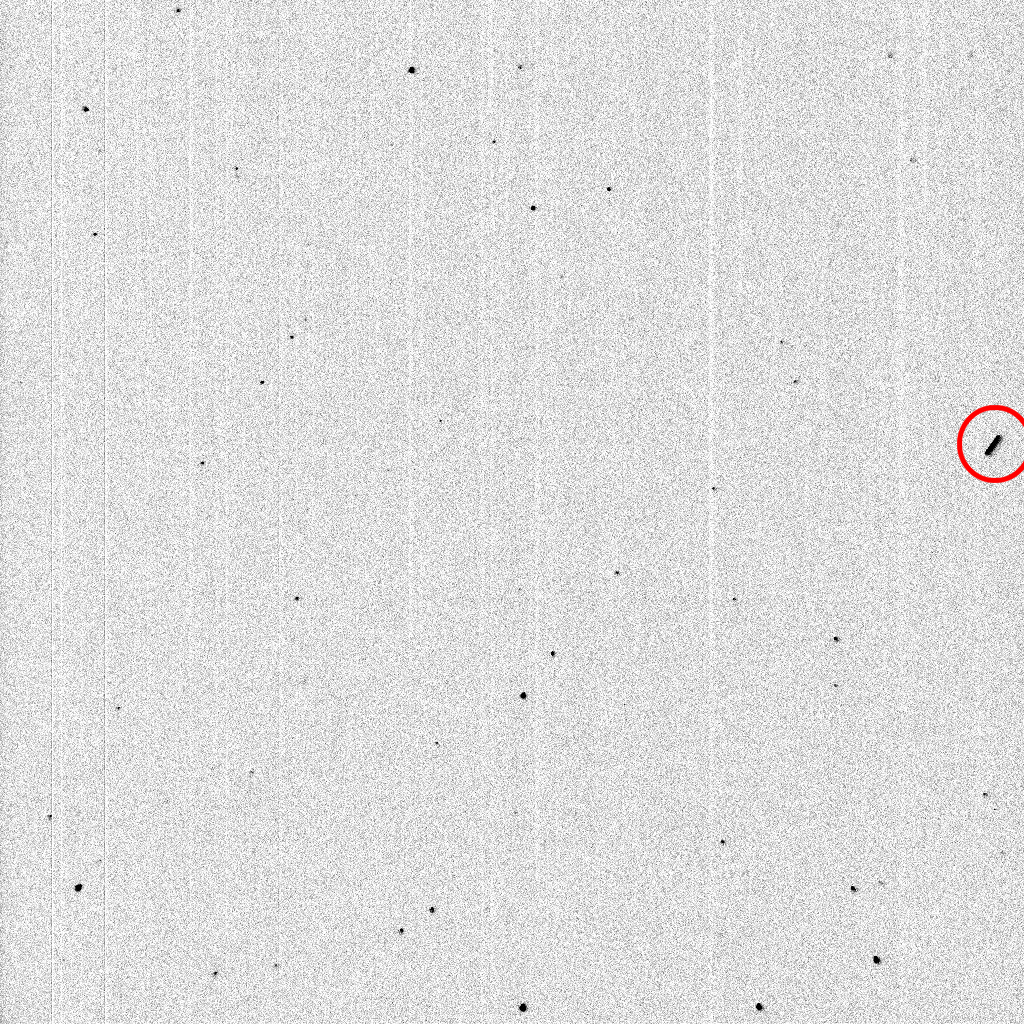
\includegraphics[width=\textwidth]{images/PointStreak1.png}
        \label{fig:pointstreak1}
    \end{subfigure}
    \hfill
    \begin{subfigure}{.3\textwidth}
        \centering
        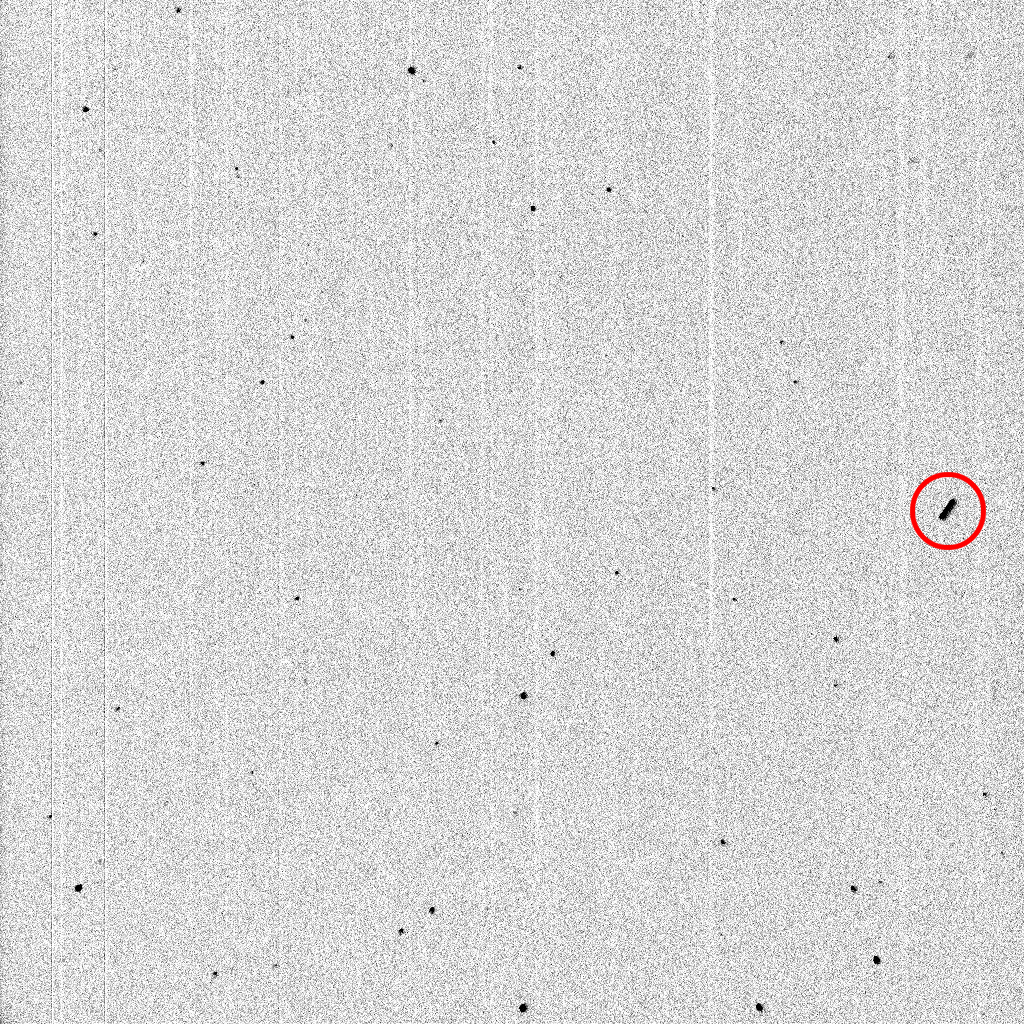
\includegraphics[width=\textwidth]{images/PointStreak2.png}
        \label{fig:pointstreak2}
    \end{subfigure}
    \hfill
    \begin{subfigure}{.3\textwidth}
        \centering
        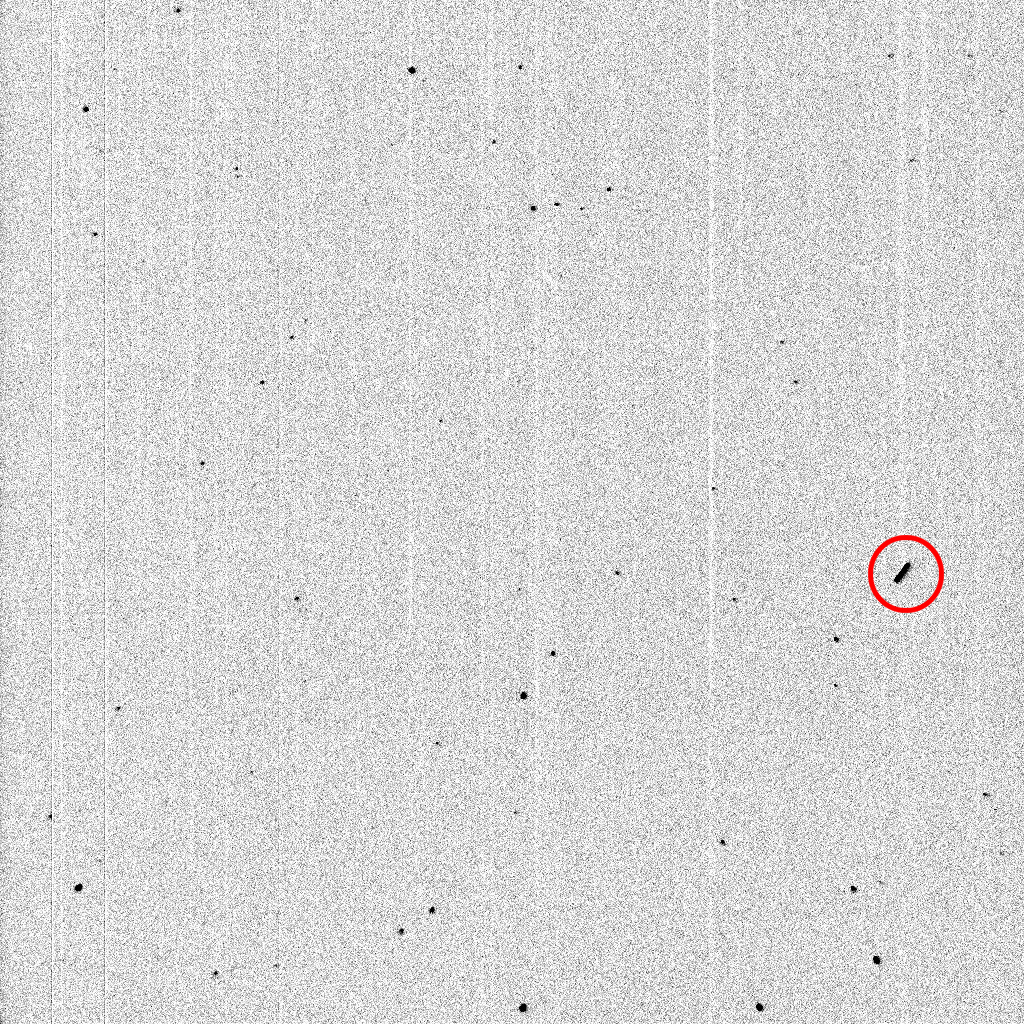
\includegraphics[width=\textwidth]{images/PointStreak3.png}
        \label{fig:pointstreak3}
    \end{subfigure}
    \hfill
    \caption{An example of series of images capturing a streak-like object and point-like stars. }
    \label{fig:pointstreak0}
\end{figure}

\subsection{Streak-like stars, point-like objects}
When the telescope is in object tracking mode, the focus is aimed at the moving object. Thus telescope is following the object matching its speed and direction. The moving object, therefore, appears as a point while stars appear as streaks. All stars will have the same length and direction of the streak-like shape. An example of one point-like object and otherwise streak-like stars are shown in the Figure \ref{fig:streakpoint0}. 

If there are more moving objects present on the frame, they can either appear as points or streaks. In case the other moving objects are moving at a similar speed and direction as the tracked object, they will also appear as points. This scenario happens when a telescope is tracking a cluster of objects. Otherwise, if other objects have different speeds and directions, they will appear as streaks but with different lengths and directions as streaks created by stars. 
This applies to both, space- and ground-based images. All these effects can influence the performance of segmentation or recognition algorithms.

\begin{figure}[!h]
    \begin{subfigure}{.3\textwidth}
        \centering
        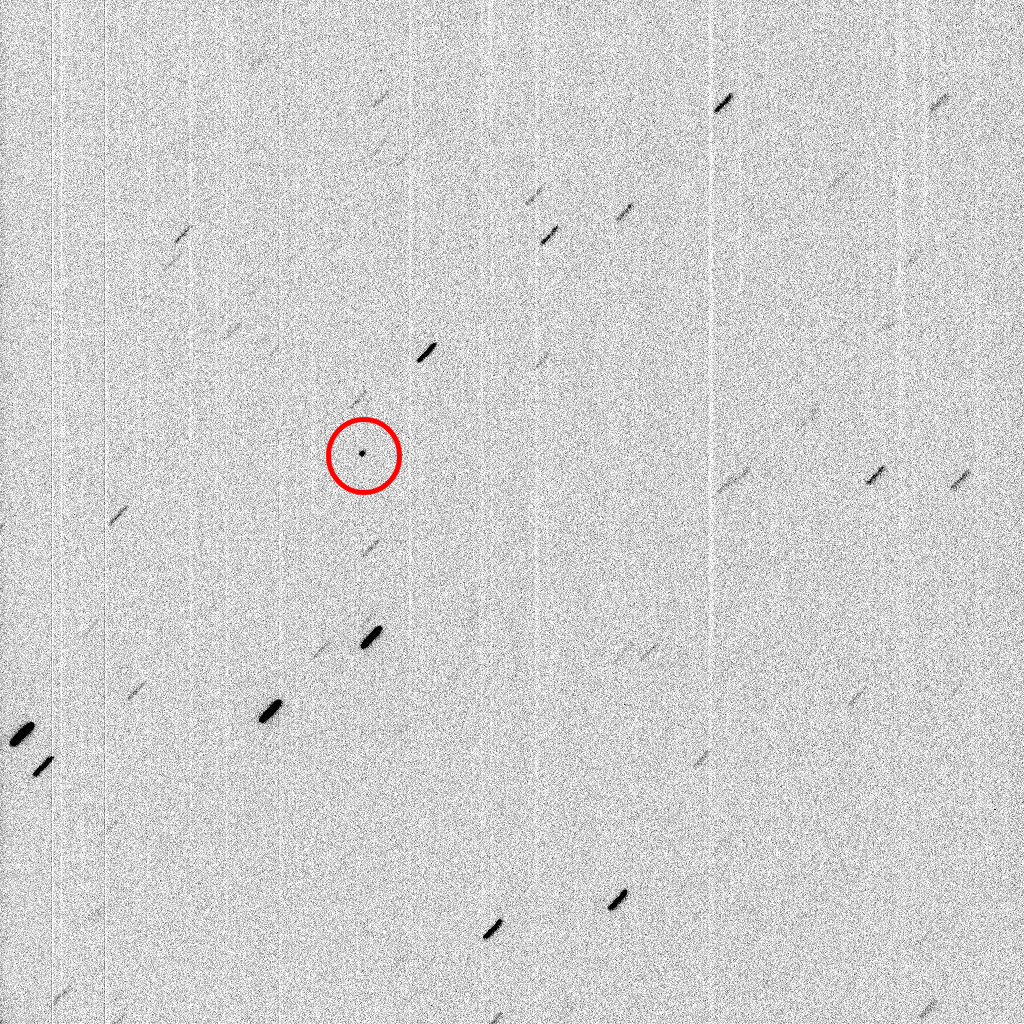
\includegraphics[width=\textwidth]{images/StreakPoint1.png}
        \label{fig:streakpoint1}
    \end{subfigure}
    \hfill
    \begin{subfigure}{.3\textwidth}
        \centering
        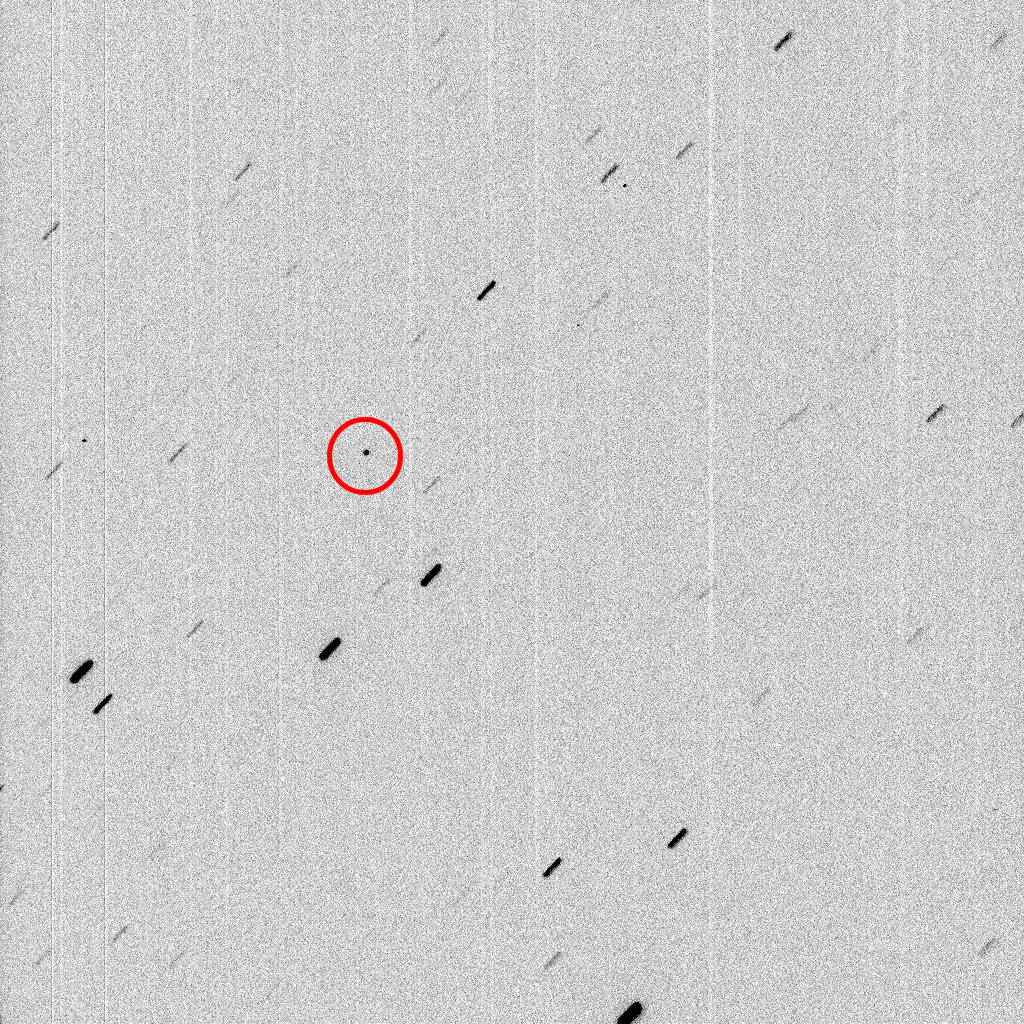
\includegraphics[width=\textwidth]{images/StreakPoint2.png}
        \label{fig:streakpoint2}
    \end{subfigure}
    \hfill
    \begin{subfigure}{.3\textwidth}
        \centering
        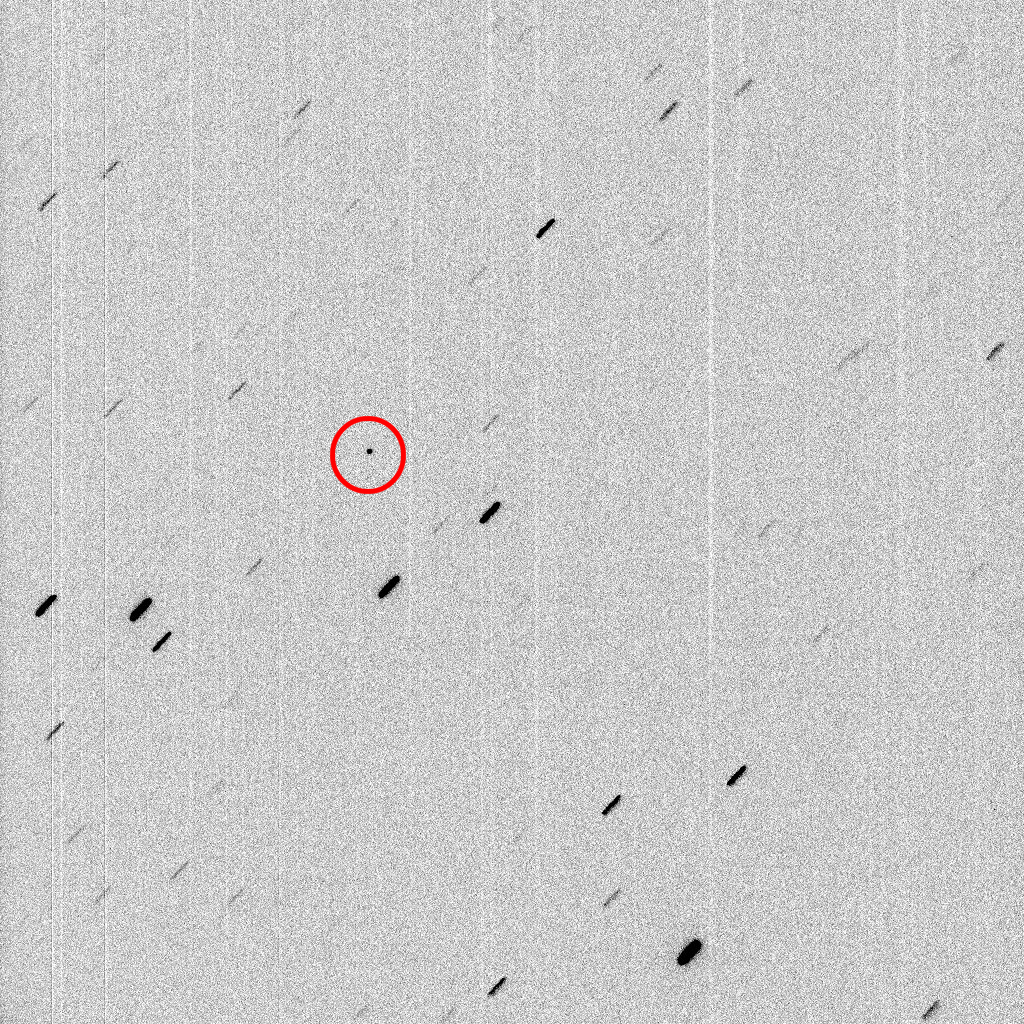
\includegraphics[width=\textwidth]{images/StreakPoint3.png}
        \label{fig:streakpoint3}
    \end{subfigure}
    \hfill
    \caption{An example of series of images capturing a streak-like stars and one point-like object. }
    \label{fig:streakpoint0}
\end{figure}

\subsection{Streak-like stars, streak-like objects}
This is a common scenario happening during the survey of the sky, when stars nor objects are being tracked, which is depicted in the Figure \ref{fig:streakstreak0}. When taking an image of the sky field during the survey, unknown objects can appear randomly, leaving streak-like features of different lengths and directions on the image. 
Stars appear as streaks in ground-based observations due to the motion of Earth and long exposure time. However streak-like stars can also be caused by the motion of the telescope in both ground and space-based observations. 

\begin{figure}[!h]
    \begin{subfigure}{.3\textwidth}
        \centering
        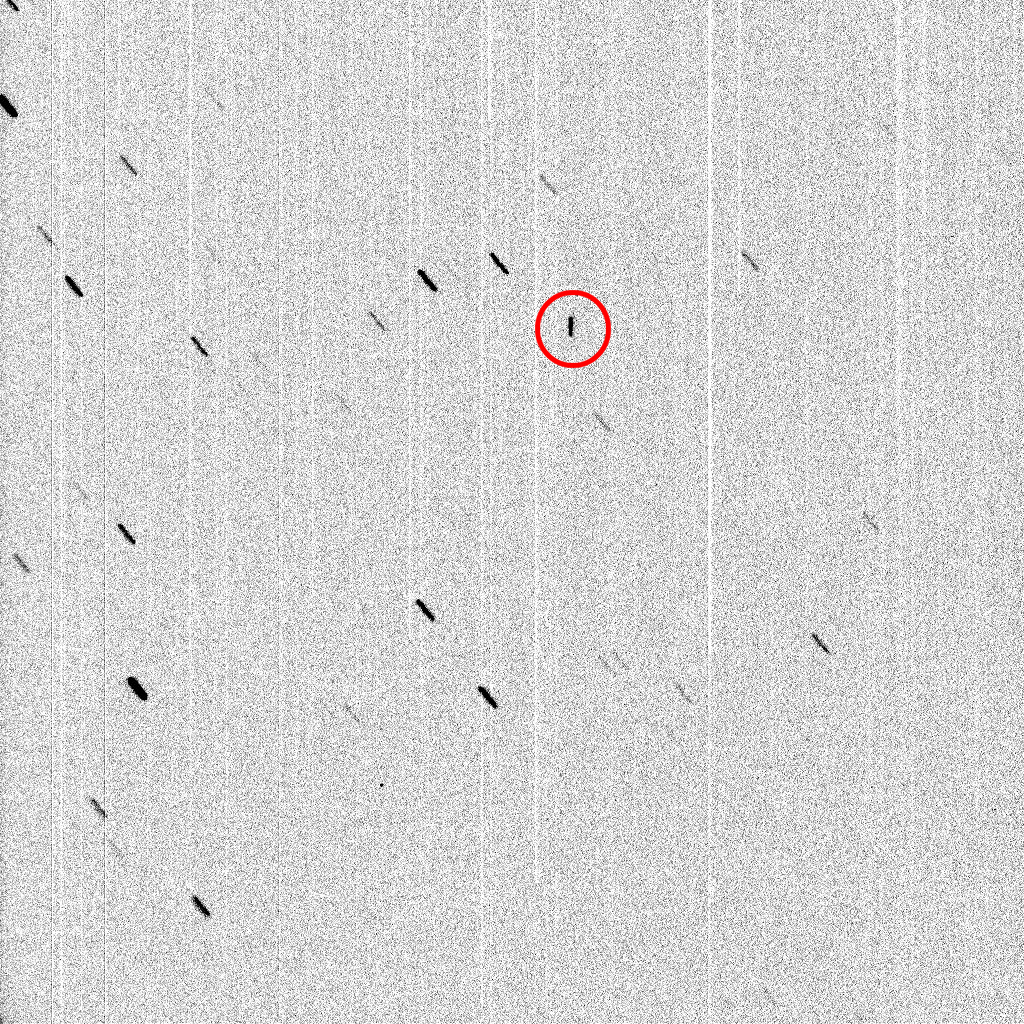
\includegraphics[width=\textwidth]{images/StreakStreak1.png}
        \label{fig:streakstreak1}
    \end{subfigure}
    \hfill
    \begin{subfigure}{.3\textwidth}
        \centering
        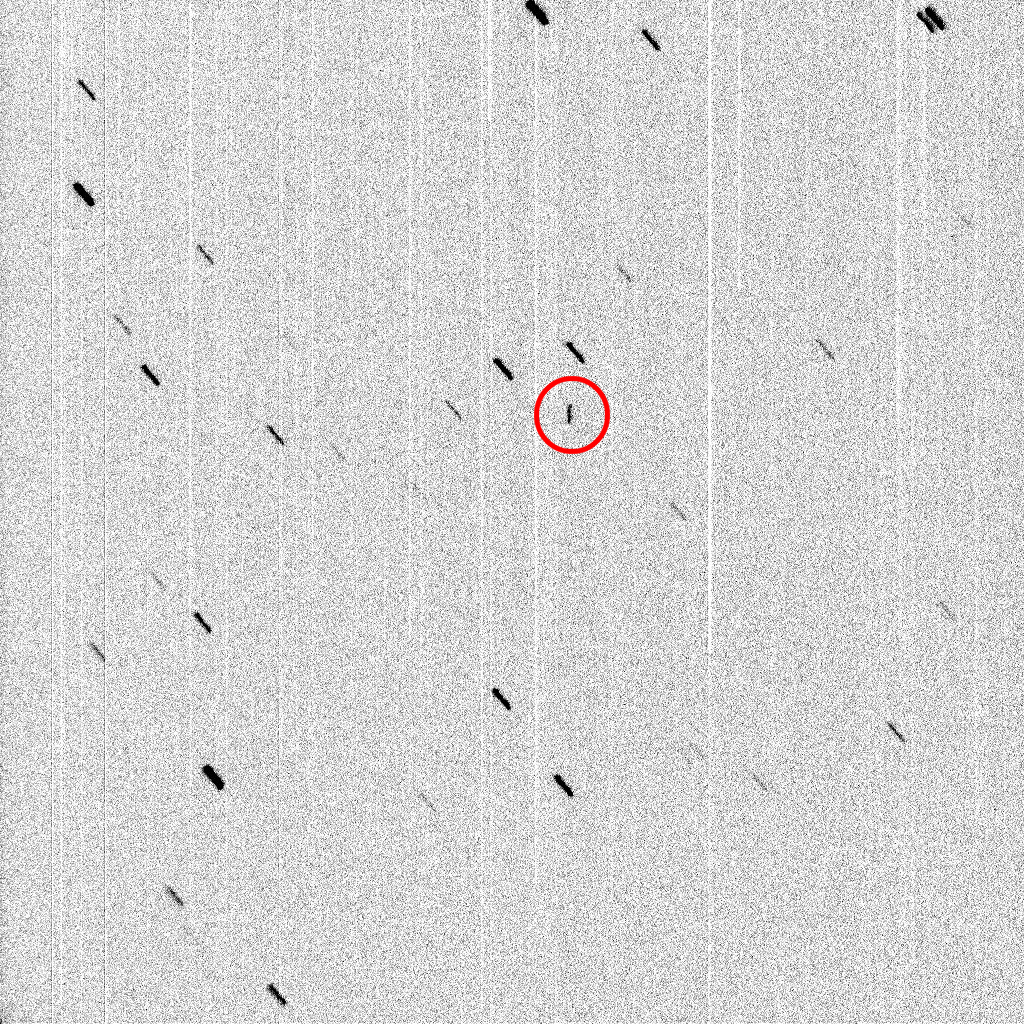
\includegraphics[width=\textwidth]{images/StreakStreak2.png}
        \label{fig:streakstreak2}
    \end{subfigure}
    \hfill
    \begin{subfigure}{.3\textwidth}
        \centering
        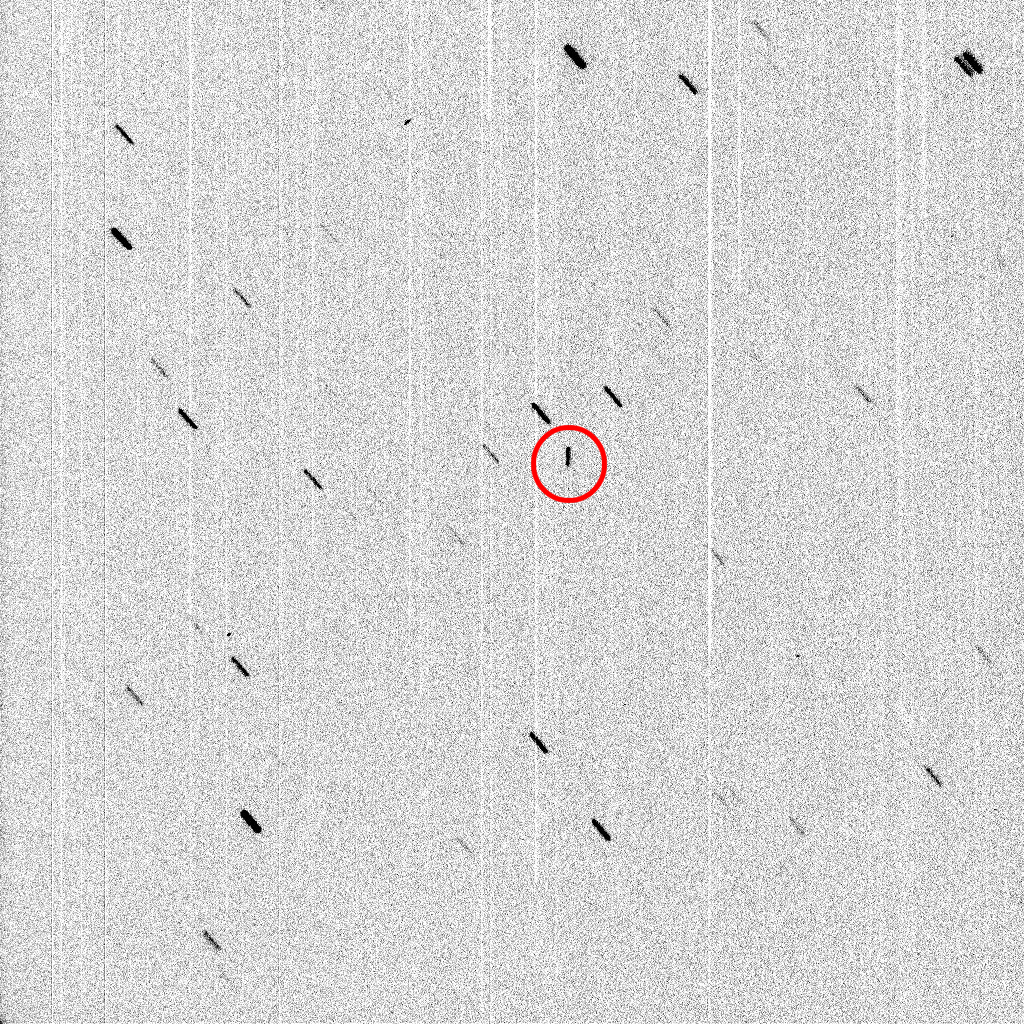
\includegraphics[width=\textwidth]{images/StreakStreak3.png}
        \label{fig:streakstreak3}
    \end{subfigure}
    \hfill
    \caption{An example of series of images capturing a streak-like stars and one streak-like object. }
    \label{fig:streakstreak0}
\end{figure}
